\exercise{Lista Doppiamente Collegata}
Si realizzi in linguaggio C++ il tipo di dato astratto \cod{Lista} mediante uso del costrutto \cod{class} del linguaggio. L'implementazione deve essere realizzata mediante puntatori ed allocazione dinamica della memoria secondo l'approccio di lista doppiamente collegata. Ogni elemento, cio�, punta contemporaneamente al precedente ed al successivo (vedi \figurename~\ref{fig:ListaDoppiamenteCollegata}). Gli elementi della lista siano uguali al tipo \cod{int} del linguaggio.

\begin{figure}
  \center
	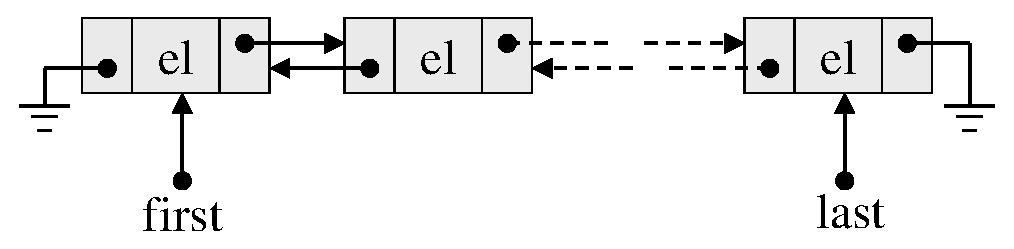
\includegraphics[width=.7\textwidth]{Esercizi/ListaDoppiamenteCollegata/Lista.eps}
	\caption{Struttura della lista doppiamente collegata}
	\label{fig:ListaDoppiamenteCollegata}
\end{figure}
        
Di seguito � riportata la specifica dei metodi pubblici da implementare per la classe \cod{Lista}.

\begin{methodslist}

\method{Lista}{\emptyset}{\emptyset} {
Costruttore.
}

\method{inserisci}{int}{\emptyset} {
Inserisce un elemento in coda alla lista.
}

\method{svuota}{\emptyset}{\emptyset} {
Svuota la lista.
}

\method{count}{\emptyset}{int} {
Conta gli elementi contenuti nella lista.
}

\method{stampaDiretta}{\emptyset}{String} {
Restituisce una stringa contenente tutti gli elementi della lista, dall'elemento di testa all'elemento di coda.
}

\method{stampaInversa}{\emptyset}{String} {
Restituisce una stringa contenente tutti gli elementi della lista, dall'elemento di coda all'elemento di testa.
}

\method{stampaAlternata}{\emptyset}{String} {
Restituisce una stringa con il contenuto della lista nel seguente ordine: primo elemento, ultimo elemento, secondo elemento, penultimo elemento, terzo elemento, terzultimo elemento...
}

Nessun metodo della classe Lista pu� utilizzare le funzionalit� di stampa (\cod{System.out}).

Si realizzi una funzione \cod{main()} che permetta di effettuare il collaudo della struttura dati realizzata.

\end{methodslist}